\documentclass[compress,aspectratio=1610]{beamer}

\usepackage{polyglossia}
\usepackage{csquotes}
\setmainlanguage{english}
\usepackage[english]{isodate}\isodate
\usepackage{appendixnumberbeamer}
\usepackage{tikz-feynman}
\usepackage{hyperref}

\usetheme[
  % Activates footline information (short title, short author).
    %fullfootline,
  % Sets a picture as the title background. If this option is not given,
  % the primary color is used to create a solid background.
    background=./graphics/forest.jpg, 
  % Whether the background is bright.
  % By default, the text on the title page will use a bright foreground
  % color. If it is given, then a dark color is used.
    %brightbackground,
  % The primary color to use for the theme.
  % Defaults to a Manchester purple
    primaryColor=666666,
  % This is intended to be a lighter version of the primary color.
    primaryLightColor=cccccc,
]{manc}

\linespread{1.1}

\title{Machine Intelligence}
\subtitle{Recent advances in AI research}
\date{\today}
\author{J. Smith}
\institute{Institute of Advanced Robotics}
\titlegraphic{
\includegraphics[width=8em]{./graphics/manchester.pdf}}

\begin{document}

\begin{frame}[plain,noframenumbering]
  \titlepage
\end{frame}

\begin{frame}
  \centering
  \usebeamercolor{palette5}%
  \tcbset{%
    colback=palette5.bg,
    colframe=palette5.bg,
    coltext=palette5.fg,
  }%
  \begin{tcolorbox}[
    before skip=30mm,
    after skip=30mm,
    boxrule=2pt,
    sharp corners,
    fonttitle=\usebeamerfont{block title},
    fontupper=\usebeamerfont{block body},
    fontlower=\usebeamerfont{block body},
    boxsep=.5mm,
    parbox=false,
    width=30em,
  ]
    \usebeamerfont{quote}
    \enquote{If a machine is expected to be infallible,\\[-0.5ex] it cannot also be intelligent.}\\
    \hfill \textup{— Alan Turing}
  \end{tcolorbox}
\end{frame}

\begin{frame}{The Manc beamer theme}
  \emph{Manc} is a minimal theme for the \LaTeX{} beamer document class that emphasizes simplicity, legibility and elegance.

  \emph{Simplicity} is achieved by a flat design that makes use of a limited palette of colors. The footline is reduced to a page counter only, getting rid of superfluous information like the author's name or the title of the presentation.
  The frame title is to be used as an \emph{accent}, ideally marking slides that contain key information.

  \emph{Legibility} is critically important for a presentation theme.
  \emph{Manc} improves legibility by using high contrasts, simplifying visual components (like blocks) and enlarging the frame counter compared to the default beamer themes.

  Several elements, like the frame title and the choice of Fira Sans as the typeface are taken from the \emph{metropolis} theme.
\end{frame}

\begin{frame}[fragile]
  \begin{columns}
    \begin{column}{0.5\textwidth}
      \begin{block}{Block}
        This is a simple block created using the \texttt{block} environment.
      \end{block}
      \begin{exampleblock}{Example block}
        This is an example block created using the \texttt{exampleblock} environment.
      \end{exampleblock}
    \end{column}
    \begin{column}{0.5\textwidth}
      \emph{Manc} replaces the default beamer blocks with boxes from the \href{https://www.ctan.org/pkg/tcolorbox}{\texttt{tcolorbox}} package.
      These can be configured in much more detail than a \texttt{beamercolorbox}
      \medskip

      Use boxes sparingly to highlight specific pieces of information (theorems, formulas, commands, …) that you want your audience to remember.\footnote[frame]{Add footnotes by using \texttt{\backslash footnote[frame]\{…\}}}
    \end{column}
  \end{columns}
\end{frame}

\begin{frame}
  \centering
  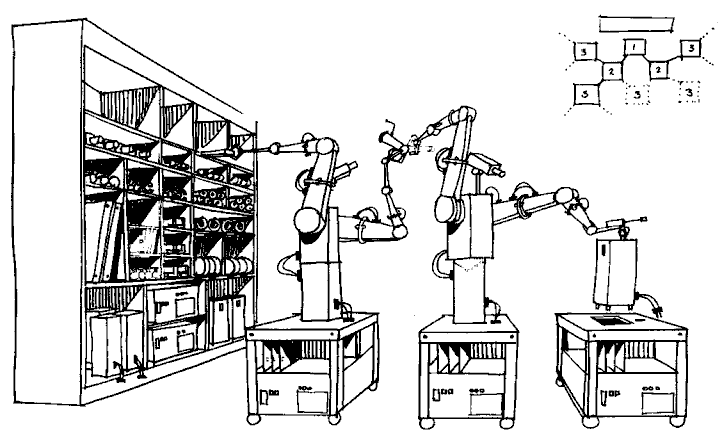
\includegraphics[width=0.9\textwidth]{./graphics/self-replicating.png}
\end{frame}

\begin{darkframe}[c,noframenumbering]
    \begin{tikzpicture}[overlay, remember picture]
    \node[anchor=center] at (current page.center) {
    \begin{beamercolorbox}[center]{title}
      \usebeamerfont{large text}Thank you for listening.
    \end{beamercolorbox}};
    \end{tikzpicture}
\end{darkframe}

%\appendix
%\begin{darkframe}
%  \centering
%  \usebeamerfont{large text} Appendix
%\end{darkframe}

\end{document}

